% GNUPLOT: LaTeX picture with Postscript
\begingroup
  \makeatletter
  \providecommand\color[2][]{%
    \GenericError{(gnuplot) \space\space\space\@spaces}{%
      Package color not loaded in conjunction with
      terminal option `colourtext'%
    }{See the gnuplot documentation for explanation.%
    }{Either use 'blacktext' in gnuplot or load the package
      color.sty in LaTeX.}%
    \renewcommand\color[2][]{}%
  }%
  \providecommand\includegraphics[2][]{%
    \GenericError{(gnuplot) \space\space\space\@spaces}{%
      Package graphicx or graphics not loaded%
    }{See the gnuplot documentation for explanation.%
    }{The gnuplot epslatex terminal needs graphicx.sty or graphics.sty.}%
    \renewcommand\includegraphics[2][]{}%
  }%
  \providecommand\rotatebox[2]{#2}%
  \@ifundefined{ifGPcolor}{%
    \newif\ifGPcolor
    \GPcolortrue
  }{}%
  \@ifundefined{ifGPblacktext}{%
    \newif\ifGPblacktext
    \GPblacktexttrue
  }{}%
  % define a \g@addto@macro without @ in the name:
  \let\gplgaddtomacro\g@addto@macro
  % define empty templates for all commands taking text:
  \gdef\gplbacktext{}%
  \gdef\gplfronttext{}%
  \makeatother
  \ifGPblacktext
    % no textcolor at all
    \def\colorrgb#1{}%
    \def\colorgray#1{}%
  \else
    % gray or color?
    \ifGPcolor
      \def\colorrgb#1{\color[rgb]{#1}}%
      \def\colorgray#1{\color[gray]{#1}}%
      \expandafter\def\csname LTw\endcsname{\color{white}}%
      \expandafter\def\csname LTb\endcsname{\color{black}}%
      \expandafter\def\csname LTa\endcsname{\color{black}}%
      \expandafter\def\csname LT0\endcsname{\color[rgb]{1,0,0}}%
      \expandafter\def\csname LT1\endcsname{\color[rgb]{0,1,0}}%
      \expandafter\def\csname LT2\endcsname{\color[rgb]{0,0,1}}%
      \expandafter\def\csname LT3\endcsname{\color[rgb]{1,0,1}}%
      \expandafter\def\csname LT4\endcsname{\color[rgb]{0,1,1}}%
      \expandafter\def\csname LT5\endcsname{\color[rgb]{1,1,0}}%
      \expandafter\def\csname LT6\endcsname{\color[rgb]{0,0,0}}%
      \expandafter\def\csname LT7\endcsname{\color[rgb]{1,0.3,0}}%
      \expandafter\def\csname LT8\endcsname{\color[rgb]{0.5,0.5,0.5}}%
    \else
      % gray
      \def\colorrgb#1{\color{black}}%
      \def\colorgray#1{\color[gray]{#1}}%
      \expandafter\def\csname LTw\endcsname{\color{white}}%
      \expandafter\def\csname LTb\endcsname{\color{black}}%
      \expandafter\def\csname LTa\endcsname{\color{black}}%
      \expandafter\def\csname LT0\endcsname{\color{black}}%
      \expandafter\def\csname LT1\endcsname{\color{black}}%
      \expandafter\def\csname LT2\endcsname{\color{black}}%
      \expandafter\def\csname LT3\endcsname{\color{black}}%
      \expandafter\def\csname LT4\endcsname{\color{black}}%
      \expandafter\def\csname LT5\endcsname{\color{black}}%
      \expandafter\def\csname LT6\endcsname{\color{black}}%
      \expandafter\def\csname LT7\endcsname{\color{black}}%
      \expandafter\def\csname LT8\endcsname{\color{black}}%
    \fi
  \fi
    \setlength{\unitlength}{0.0500bp}%
    \ifx\gptboxheight\undefined%
      \newlength{\gptboxheight}%
      \newlength{\gptboxwidth}%
      \newsavebox{\gptboxtext}%
    \fi%
    \setlength{\fboxrule}{0.5pt}%
    \setlength{\fboxsep}{1pt}%
\begin{picture}(7200.00,5040.00)%
    \gplgaddtomacro\gplbacktext{%
      \csname LTb\endcsname%%
      \put(228,504){\makebox(0,0)[r]{\strut{}$-10$}}%
      \put(228,1080){\makebox(0,0)[r]{\strut{}$-9$}}%
      \put(228,1656){\makebox(0,0)[r]{\strut{}$-8$}}%
      \put(228,2232){\makebox(0,0)[r]{\strut{}$-7$}}%
      \put(228,2807){\makebox(0,0)[r]{\strut{}$-6$}}%
      \put(228,3383){\makebox(0,0)[r]{\strut{}$-5$}}%
      \put(228,3959){\makebox(0,0)[r]{\strut{}$-4$}}%
      \put(228,4535){\makebox(0,0)[r]{\strut{}$-3$}}%
      \put(648,284){\makebox(0,0){\strut{}$-3$}}%
      \put(1224,284){\makebox(0,0){\strut{}$-2$}}%
      \put(1800,284){\makebox(0,0){\strut{}$-1$}}%
      \put(2375,284){\makebox(0,0){\strut{}$0$}}%
      \put(2951,284){\makebox(0,0){\strut{}$1$}}%
      \put(3527,284){\makebox(0,0){\strut{}$2$}}%
    }%
    \gplgaddtomacro\gplfronttext{%
      \csname LTb\endcsname%%
      \put(-388,2519){\rotatebox{-270}{\makebox(0,0){\strut{}$log_{10} \left|x-x_0 \right|$}}}%
      \put(1943,-46){\makebox(0,0){\strut{}$log_{10} \tau$}}%
    }%
    \gplgaddtomacro\gplbacktext{%
      \csname LTb\endcsname%%
      \put(3540,504){\makebox(0,0)[r]{\strut{}}}%
      \put(3540,1008){\makebox(0,0)[r]{\strut{}}}%
      \put(3540,1512){\makebox(0,0)[r]{\strut{}}}%
      \put(3540,2016){\makebox(0,0)[r]{\strut{}}}%
      \put(3540,2520){\makebox(0,0)[r]{\strut{}}}%
      \put(3540,3023){\makebox(0,0)[r]{\strut{}}}%
      \put(3540,3527){\makebox(0,0)[r]{\strut{}}}%
      \put(3540,4031){\makebox(0,0)[r]{\strut{}}}%
      \put(3540,4535){\makebox(0,0)[r]{\strut{}}}%
      \put(3960,284){\makebox(0,0){\strut{}$-3$}}%
      \put(4536,284){\makebox(0,0){\strut{}$-2$}}%
      \put(5112,284){\makebox(0,0){\strut{}$-1$}}%
      \put(5687,284){\makebox(0,0){\strut{}$0$}}%
      \put(6263,284){\makebox(0,0){\strut{}$1$}}%
      \put(6839,284){\makebox(0,0){\strut{}$2$}}%
      \put(6971,504){\makebox(0,0)[l]{\strut{}$-18$}}%
      \put(6971,1008){\makebox(0,0)[l]{\strut{}$-16$}}%
      \put(6971,1512){\makebox(0,0)[l]{\strut{}$-14$}}%
      \put(6971,2016){\makebox(0,0)[l]{\strut{}$-12$}}%
      \put(6971,2520){\makebox(0,0)[l]{\strut{}$-10$}}%
      \put(6971,3023){\makebox(0,0)[l]{\strut{}$-8$}}%
      \put(6971,3527){\makebox(0,0)[l]{\strut{}$-6$}}%
      \put(6971,4031){\makebox(0,0)[l]{\strut{}$-4$}}%
      \put(6971,4535){\makebox(0,0)[l]{\strut{}$-2$}}%
    }%
    \gplgaddtomacro\gplfronttext{%
      \csname LTb\endcsname%%
      \put(3540,2519){\rotatebox{-270}{\makebox(0,0){\strut{}}}}%
      \put(5255,-46){\makebox(0,0){\strut{}$log_{10} \tau$}}%
      \csname LTb\endcsname%%
      \put(5519,3900){\makebox(0,0)[l]{\strut{}$\lambda = 10$}}%
      \csname LTb\endcsname%%
      \put(5519,4120){\makebox(0,0)[l]{\strut{}$\lambda = 1$}}%
      \csname LTb\endcsname%%
      \put(5519,4340){\makebox(0,0)[l]{\strut{}$\lambda = 0,1$}}%
    }%
    \gplbacktext
    \put(0,0){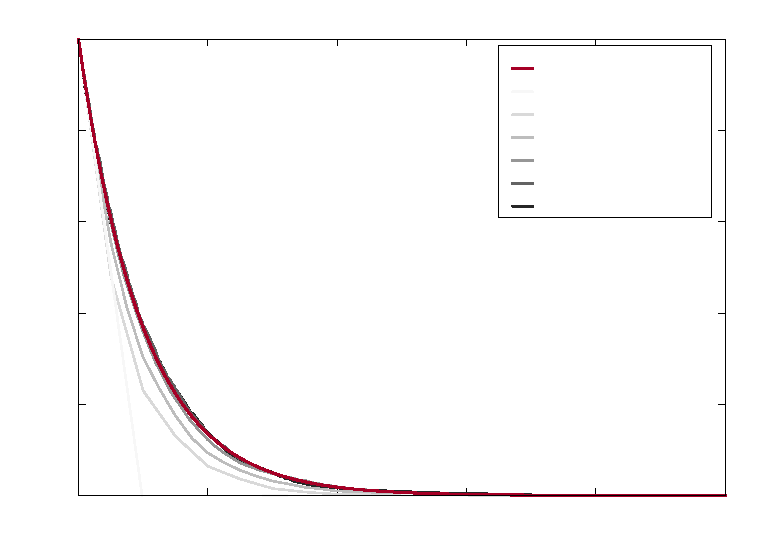
\includegraphics{graf6}}%
    \gplfronttext
  \end{picture}%
\endgroup
